% $Id: usbmasss.tex 10138 2022-06-04 23:46:50Z mskala $

%
% USB mass storage and FAT filesystem
% Copyright (C) 2022  Matthew Skala
%
% This program is free software: you can redistribute it and/or modify
% it under the terms of the GNU General Public License as published by
% the Free Software Foundation, version 3.
%
% This program is distributed in the hope that it will be useful,
% but WITHOUT ANY WARRANTY; without even the implied warranty of
% MERCHANTABILITY or FITNESS FOR A PARTICULAR PURPOSE.  See the
% GNU General Public License for more details.
%
% You should have received a copy of the GNU General Public License
% along with this program.  If not, see <http://www.gnu.org/licenses/>.
%
% Matthew Skala
% https://northcoastsynthesis.com/
% mskala@northcoastsynthesis.com
%

\chapter{USB mass storage and filesystem (usbmass.s)}

The mass storage driver's only application in the current firmware is to
read a firmware image file from a USB mass storage device (which would
probably be a flash drive) and store it in the SRAM chip for the code in
loader.s to use.  Actually doing that requires multiple layers of driver
code: establishing low-level communication with the mass storage device's
USB bulk endpoints; sending SCSI commands sent over that communication
channel; handling the partitioning of the drive, if any; and decoding the
FAT filesystem that will be stored either in a partition or on the drive as
a whole.  All these layers are included in the file usbmass.s.  Some future
or modified firmware might be able to reuse parts of this code for other
applications.

\section{USB mass storage overview}

The USB standards allow for mass storage devices to have many different
kinds of interface, but USB flash drives almost universally use just one:
the \emph{bulk-only SCSI} interface.  This interface is basically just a USB
wrapper around SCSI commands.  The SCSI commands then expose a simple
interface where the drive is regarded as an array of blocks indexed from 0
up to whatever size, and the host can request a read or a write of however
many blocks starting at a given block number.  Block size is variable in
principle but basically always 512 bytes in practice (the Gracious Host code
is designed to support powers of two from 256 to 4096, though the FAT
filesystem may require 512 minimum).  Index length, determining the number
of blocks allowed, may be up to 64 bits when using the longest form of the
SCSI READ command, but the Gracious Host firmware uses the READ (10) command
with a maximum index length of 32 bits, corresponding to 2T drive capacity
when the blocks are 512 bytes.

Sending a command to the mass storage device on the bulk-only SCSI interface
goes in three stages.  First, the host sends a \emph{Command Block Wrapper}
(CBW) to the device's bulk out endpoint.  The CBW is 31 [sic] bytes long,
with little endian fields in it, and it contains an unaligned 16-byte field
for the SCSI \emph{Command Descriptor Block} (CDB), padded to 16 bytes in
the common case where the CDB is smaller.  The CDB is as defined by the SCSI
standard.  It contains big endian fields, which tend to be 16-bit aligned
from the CDB's point of view but end up unaligned in the CBW because of the
CDB's unaligned start address.

After sending the CBW, the host transfers as much data as the command
requires, through the device's bulk in or out endpoints as appropriate. 
That might involve multiple USB transactions because of the 512 byte per
transaction limit of full-speed USB, but the data amount could be as small
as zero in the case of a SCSI command that needs no data beyond the CDB.

Finally, the host receives a \emph{Command Status Wrapper} (CSW) from the
device's bulk in endpoint.  The CSW is 13 bytes long and reports whether the
command was successful or not.

To use the bulk in and out endpoints both for the wrapper structures and the
data transfer like this, creates some concern about the device and host
possibly falling out of synchronization.  To help address that concern, the
CBW and CSW each start with magic numbers, and the CBW contains a 32-bit tag
field which the host can set arbitrarily and the device is supposed to
repeat back in the CSW.  The Gracious Host firmware uses the PRNG API from
utils.s to choose tag values.  When the host reads a 13-byte chunk of data
that it thinks ought to be the CSW, it can check that the magic number is
correct for a CSW at all, and that the tag matches the one it sent in the
CBW, and if both matches succeed then it can guess that the synchronization
is probably correct.

SCSI offers a wide range of commands from basic block read and write to
esoteric copy-protection commands for outdated movie-distribution systems. 
There does not seem to be any standard for exactly which ones a USB flash
drive will or will not support.  The USB standards only go as far as how to
get SCSI commands to and from the drive and then leave the rest to the SCSI
standard.  SCSI itself provides some capability for auto-detecting which
commands a device can support, but it is not clear that every USB flash
drive even supports the commands to do that autodetection properly.  The
Gracious Host uses only the READ CAPACITY (10) and READ (10) commands, which
are a bare minimum set expected to be supported on all devices that it could
possibly work with.  The parenthesized (10) in the command names refers to
the length of the CDB for these commands (ten bytes); SCSI often defines
multiple forms of a given command with different CDB lengths, usually to
allow for larger fields to support larger drives in the longer CDBs.

\section{Partition and FAT structure}

The Gracious Host firmware looks for an update image:
\begin{itemize}
  \item in a file named FIRMWARE.FRM,
  \item in the root directory of a FAT filesystem,
  \item \emph{either} written directly to the flash drive starting at block
    0,
  \item \emph{or} contained in a primary partition described by an MS-DOS-style
    partition table in block 0.
\end{itemize}

The firmware makes a few simplifying assumptions to reduce the complexity of
searching for the file.  It does not write to the filesystem; it does not
handle extended partitions; it does not handle subdirectories; and it does
not handle long filenames.  It should still work on a flash drive which has
any or all of those things, but the update image file must meet the criteria
above to be found.  On the other hand, the firmware is intended to handle
all of FAT12, FAT16, and FAT32, including some weird variants with
nonstandard layout to the extent that that does not significantly increase
the complexity of handling the most-expected cases.  FAT32 is expected to be
the most common and is the best tested.

Here's a brief description of how the on-disk data structures work, which
may help with understanding the more code-oriented description of the driver
code.

First:  hard drives formatted for MS-DOS, and Windows later adopted the
convention, usually start with the first 512-byte block defined to contain a
\emph{partition table}, which describes up to four non-overlapping ranges of
the subsequent blocks, with a little bit of metadata attached to each range. 
These are called \emph{primary partitions}.  DOS and Windows traditionally
show each partition as a separate drive letter, so one might have a single
physical hard disk that appears in the operating system as drives C:, D:,
and E:.  Each partition is formatted separately with a filesystem, and it is
even possible to put different operating systems' formats on different
partitions.  Dual boot configurations on PCs would often do that.

There can only be at most four primary partitions, but it quickly became
apparent that having more than four partitions on a disk might be useful. 
Some variants of DOS put a larger table in the first block of the disk, but
with regular MS-DOS there is not really enough space to store descriptions
for more them four partitions in the 512-byte first block, especially not
when (as is the case on some PC hardware) that block also needs to contain
some boot loader code.  So to allow more partitions, they added a concept to
the format of having one of the four primary partitions be marked as the
\emph{extended partition}.  Then a further partition table (not in the same
format) could describe lower-level partitions inside the extended partition,
an effectively unlimited number of them.

USB flash drives are usually formatted with a partition table in the first
block, and that partition table describing exactly one primary partition
covering the rest of the drive, with a FAT filesystem inside the partition. 
Another reasonably common setup is to have no partition table at all, and
the FAT filesystem just covering the entire drive with its first block in
the drive's first block.  The Gracious Host is designed to handle at least
those two cases.  It can also handle some others -- such as more than one
primary partition and the relevant FAT filesystem inside one of them -- but
it cannot handle every unusual case that a PC's operating system might
handle.

The term \emph{FAT filesystem} refers to the data structure that stores a
tree of files with names and directory paths inside what on DOS or Windows
would be one drive letter.  This data structure is more or less directly
descended from the high-level format that the first versions of MS-DOS used
on floppy disks, enhanced and extended with the features needed for the much
larger storage devices of modern PCs.

The FAT filesystem views the disk, or the subrange of the disk that it
covers if operating inside a partition, as an array of what it officially
calls \emph{logical sectors} but I prefer to call \emph{FAT blocks}.  A FAT
block is a power-of-two number of bytes that may or may not match the size
of a \emph{drive block} as used by SCSI.  The Gracious Host firmware is
designed to work with FAT blocks larger or smaller than drive blocks, and
either of those cases is \emph{possible}, but in practice it is likely that
the FAT blocks and drive blocks will both be equal to 512 bytes, and some
other implementations fail if the sizes do not match.  The size of a FAT
block can possibly be chosen during formatting (for instance, with the -S
option to Linux mkfs.fat).  The size of a drive block is normally fixed by
the hardware.

The first FAT block of the filesystem (called the \emph{superblock} in Unix
terminology and in the Gracious Host code, though DOS and Windows would
probably call it something else) contains metadata about the filesystem,
identifying that this is a FAT filesystem, what version it is, how big it
is, and the locations and sizes of some other structures.  There may be some
blocks near the start reserved for various purposes like boot loader code,
and on some FAT filesystems (for instance, those created for temporary
storage by Windows Update), these reserved blocks may cover a considerable
amount of storage.

The next two significant things in the filesystem are the root directory and
what I'm calling the \emph{FAT per se} -- that is, the array named the File
Allocation Table (FAT) that also lends its name to the entire filesystem. 
FAT filesystems exist in variants called FAT12, FAT16, and FAT32, referring
to the number of bits per entry in the FAT per se.  Some of the information
in the superblock indicates which of these applies, and some details of the
other structures, in particular the way the root directory is stored, vary
depending on the variant.  For FAT12 and FAT16, the root directory is just
an array of directory entries (\emph{dirents}) in reserved FAT blocks near
the start of the filesystem, with a starting point and length described in
the superblock.  FAT32's root directory is a little more complicated and
discussed below.

Usually, there is a second copy of the FAT per se, either as a simple backup
or to support clever journalling schemes that update one completely and then
the other and can recover from an interrupted update operation.  Rarely,
there may be three or more copies.  The Gracious Host only looks at the
first one.

The remainder of the filesystem, after the special structures at the start,
is divided into \emph{clusters}, which are larger blocks formed out of FAT
blocks.  Clusters are the smallest units of space allocation and there is an
entry for each cluster in the FAT per se, so there is a tradeoff between
using smaller clusters for better allocation efficiency, and larger clusters
for fewer FAT entries.  Each cluster is some power-of-two number of FAT
blocks, with the number of FAT blocks per cluster specified in the
superblock.  They tend to be larger on larger disks, with a size of 8K per
cluster (16 FAT blocks of 512 bytes each, per cluster) being fairly common. 
Clusters larger than that are less common and may be unsupported by some
implementations; 16K is usually safe but the exact upper bound is not very
well-defined.  The files; subdirectories; and on FAT32, the root directory;
are stored in the clusters.

Files (with directories being special files) are stored in linked lists of
clusters.  From somewhere (where, depends on the type of object) you get the
number of the first cluster.  The first cluster's worth of data in the file
is in that cluster number.  Then you take the cluster number as an index
into the entries of the FAT per se.  The entry at the specified location
tells you the number of the \emph{next} cluster, or a reserved value,
effectively a null pointer, indicating that that was the last cluster.  If
there is a next cluster, you get more data from the corresponding cluster,
then go back to the FAT per se to get the cluster number for the third
cluster of the object; and so on.  There are other reserved values, which
should never appear within a file chain, for currently-unused clusters
(available for writing new files or expanding existing ones) and defective
clusters where the system should not attempt to store data.

Directories are arrays of dirents, each representing a file or an empty slot
where a file could be stored, with metadata like the file's name, time
stamp, and size in bytes (necessary for knowing how much of the last cluster
in the chain to actually use).  The basic FAT dirent only has 11 bytes for
the filename (stylized for display as an 8-character ASCII name followed by
a 3-character extension, like FIRMWARE.FRM); enhancements in later
versions of the format involve storing an abbreviated name in the regular
dirent and then using special dirents that older systems will not recognize
as files, to store chunks of a longer filename.  If the filesystem has
subdirectories, then those are stored like files with some bits set to
indicate they are actually subdirectories, and then the content of such a
file, inside its chain of clusters, will be more dirents for the files and
lower-level subdirectories in the subdirectory.

The root directory for FAT12 or FAT16 is in a fixed-length chunk of reserved
FAT blocks near the start of the filesystem.  For FAT32, the root directory
is stored in a chain of clusters, as if it were a file or subdirectory,
starting in a cluster number specified in the superblock.  Subdirectories
are stored in chains of clusters, starting at clusters specified in their
parent directories.  To read the data of a file, in general we must find the
directory containing it, read through that to find the corresponding dirent
for the file, and then the dirent will contain the starting cluster number
of the file.  Reading through the file (or through a directory that is
stored in clusters) requires following the chain of pointers through the FAT
per se.

The driver code makes use of a data structure it calls a CABA:  a Cluster
And Block Address.  The CABA points to a FAT block within a cluster.  It is
six bytes long.

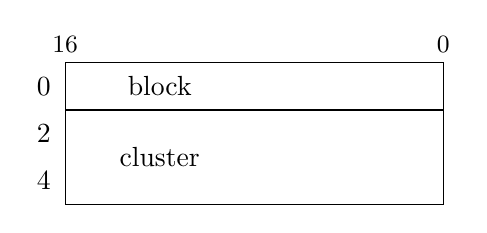
\begin{tikzpicture}[scale=0.3]
  \draw (0,0) rectangle (16,-6);
  \draw (0,-2) -- (16,-2);
%
  \node[anchor=east] at (-0.2,-1) {0};
  \node[anchor=east] at (-0.2,-3) {2};
  \node[anchor=east] at (-0.2,-5) {4};
  \node[anchor=south] at (0,0) {\small 16};
  \node[anchor=south] at (16,0) {\small 0};
%
  \node at (4,-1) {block};
  \node at (4,-4) {cluster};
\end{tikzpicture}

The fields are defined as follows.

\begin{description}
  \item[block] index of the block within the cluster; for instance, with
    four FAT blocks per cluster, this field is in the range 0--3.
  \item[cluster] 32-bit number of the cluster within the filesystem,
    using the FAT filesystem's standard indexing in which the first valid
    cluster is number 2.
\end{description}

Some of the driver's internal subroutines take a pointer to a CABA as an
argument.

Below the level of the CABA, the firmware makes use of a buffer pool that
caches either FAT blocks or drive blocks.  The init\_buffer\_pool subroutine
initializes or reinitializes this pool, using memory allocated on the stack,
as many buffers as will fit while leaving a small allowance for other uses
of the stack at the end of RAM.  Requests for a block through
get\_fat\_block and get\_drive\_block check the cache first and go to the
USB device only if the block was not already cached, with a simple cache
replacement policy.

\section{USB device simulation (overview)}

Testing the FAT filesystem code on real hardware is tricky, especially with
respect to unusual barely-standard flash drive hardware and FAT parameters,
because on top of the usual issues of trying to single-step the
microcontroller without the USB device giving up, unusual hardware is by
nature hard to find.  Generating FAT images with oddball parameters is a
little easier because that can be done in software, but doing it reproducibly
is not easy on every development machine, and loading the oddball images
into the barely-standard flash hardware may present additional difficulties.

So to make debugging easier, the USB mass storage driver has a built-in
simulation feature.  When SIMULATE\_USB\_MASS is defined in config.inc with
an integer from 1 to 6, after boot-up instead of going into the main loop in
firmware.s, the firmware will jump into the USB mass storage driver; and
whenever it tries to read from the mass storage device, it will instead read
canned data from program memory.  The file simdrive.inc sets up the program
memory data for one of six test cases selected by the SIMULATE\_USB\_MASS
value as follows.

\begin{description}
  \item[1] 32G USB stick with FAT32 filesystem in a partition, 512-byte
    drive and FAT blocks, 16K cluster size, some unusal parameters because
    it was formatted by the Windows 10 upgrade process, target file
    unfragmented but deep in the partition so that cluster indices will exceed
    16-bit range.
  \item[2] 80M drive with FAT32, 512-byte drive and FAT blocks, 512-byte
    cluster size, target file heavily fragmented.
  \item[3] 20M drive with FAT16, 512-byte drive and FAT blocks, 1K clusters.
  \item[4] 80M drive with FAT16, 512-byte drive blocks, 2K FAT
    blocks, 8K clusters.
  \item[5] 360K drive with FAT12 (simulating floppy disk), 512-byte drive and
    FAT blocks, 1K clusters.
  \item[6] 1440K drive with FAT12, 2K drive blocks, 1K FAT blocks, 1K
    clusters.
\end{description}

There is a list of blocks hardcoded into the simdrive.inc file for each test
case, and the data for each block of the FAT infrastructure is loaded from
files named like fat32a.bin, fat32b.bin, fat16a.bin, and so on.  These files
are provided in the source package inside simdrive-images.zip.  Be aware
that that file is heavily compressed, containing about 182M of image files
mostly full of zeroes; unpacking it is only recommended if you actually
intend to use the drive-simulation feature.
The data bytes for the simulated firmware image file are extracted not from
the disk images but from simdrive.bin, which is a copy of the current
firmware automatically created by the Makefile as a side effect of doing a
regular build.

When the firmware attempts to read a block in simulation mode, it scans the
list of block numbers, and if the desired block number is found, it then
reads the associated data from program memory.  The consequence of this
design is that the list in simdrive.inc of blocks to be stored for a test
case needs to contain all the blocks that the firmware will attempt to read
while running the test case.  If firmware bugs cause it to read unexpected
blocks, or if the fat*.bin file contents change in a way that points it to
unanticipated block numbers, then the simulated drive will be unable to
return a result for a read call and the firmware will crash in the debugger. 
But as supplied, with the fat*.bin files included with the source, all six
test cases should be able to run as far as starting the loader.

The loader cannot actually succeed with a simulated USB flash drive because
if running in Microchip's simulator, there will be no SRAM to provide data
to the loader; and even if running in real hardware, the entire firmware
image is not actually stored in the simulated drive (simdrive.inc just
folds over the first 8K bytes to make up the size), and so a CRC32 checksum
will probably fail in the loader.  The simulation is only intended for
checking the FAT code.

The file fat32a.bin was created by hand-selecting a few blocks from a FAT
image full of Windows update files that I can't share in full (and it would
be 32G anyway, which is a lot to share).  The others were created by the
included mksimdrives script and in principle could be re-created by running
that script again.  But be careful: first, this script must run as root and
on a Linux system, because it mounts and unmounts loopback image files using
Linux-specific commands.  Also, although it is fairly consistent on my
installation as long as the firmware image size does not change, it is quite
likely that re-running it after any development has occurred will produce
slightly different images, with file blocks in different locations within
the images, so that the block numbers in simdrive.inc may need to be patched
up by hand for the test cases to work after re-running it.  The mksimdrives
script is included primarily for reference and actually running it is not
really recommended.  At the very least, \emph{as with any root script}, you
should go through it, edit it to put in your preferred pathnames, and make
sure you understand how it works, before running it as root on your system.

The remainder of this chapter describes the source code of the driver, which
talks to the USB flash drive using the USB Mass Storage and SCSI commands,
reads drive blocks, breaks or joins them into FAT blocks, and decodes the
FAT filesystem format.  The sections of documentation are arranged in the
same sequence as the code, which may not be the easiest sequence for
understanding the layers of abstraction involved.  Refer back to the
conceptual material above as needed for the description of the data
structures.

\section{TPL entry and RAM data}

Like most Gracious Host per-device drivers, the source file starts with a
TPL entry and some data structures defined in the common data area.  The TPL
entry for this driver is set up to recognize devices exposing an interface
descriptor of USB class 8 (``mass storage''), subclass 6 (``SCSI''),
protocol 80 (``bulk-only'').

The common data area is laid out as required by FIND\_IN\_OUT\_ENDPOINTS
(reused from qwerty.s), with pointers to the first in and out endpoints
at the very start of the common data followed by an array of EP data
structures.  In this case there are just two EPs in the array; we expect the
device to expose exactly one in and one out endpoint.  After that the code
reserves separate IRPs for CBW, CSW, and data transfers, so that we can
avoid needing to reinitialize a shared IRP for these different uses.  See
the USB mass storage overview above.

The rest of the common data variables generally relate to block buffers and
decoding the partition table and FAT filesystem.  They will be described as
they are used.

\section{Driver init}

Unlike most per-device drivers, this one has no ``main loop''; it
unconditionally does its work and then starts the loader instead of
retaining control indefinitely.  At the entry point usbmass\_driver, it
starts by calling USB\_CONFIGURE\_DEVICE to select the configuration and
then FIND\_IN\_OUT\_ENDPOINTS (from qwerty.s) to determine which nedpoint is
the input and which is the output.  Both must exist; if not, the driver
terminates with a THROW.

This driver uses the PRNG subsystem (for CBW/CSW tags), so it calls
START\_CRC to initialize that, and makes a PRNG\_HASH\_TIMERS call at the
start as well to make sure there is at least a little bit of entropy in the
pool.

The first SCSI command sent to the flash drive is READ CAPACITY (10), which
gets the drive's block size and number of blocks.  The code calls
set\_up\_cbw with appropriate parameters to set up the data structures for
this command, then wait\_and\_hash to send it to the device.  These
subroutines are defined later in the file.  The data block for this command
is eight bytes; the code calls transfer\_and\_check\_csw to complete the
command.  If SIMULATE\_USB\_MASS is defined, then a block of code at this
point fills in simulated values for the block size and number of blocks.

Next are some checks for acceptable values returned from the drive.  Drives
greater than $2^{32}$ blocks in size (2T if the blocks are 512 bytes) need a
different command to read their true sizes; they return a last-block index
of 0xFFFFFFFF with READ CAPACITY (10).  The code checks for that value and
THROWs if it is seen; the Gracious Host does not work with drives bigger
than the 32-bit limit.  Next, it confirms that the block size is less than
64K.

The initialization section ends with a call to init\_buffer\_pool, which
sets up the cache to use a block size matching the drive's.  This decision
may be changed later if FAT blocks turn out to differ in size from drive
blocks.

\section{Reading the FAT superblock}

The driver will look for a FAT superblock in up to five places:  block~0,
and the four blocks pointed to by the primary partition table entries, which
are stored in block~0.  In order to reuse the code that checks for a
superblock, these checks are structured so that ``starting in block~0
without a partition table'' is treated as an entry at index $-$1.  The
initialization code sets the partition\_table variable, a 32-bit block index
for the start of the partition currently under consideration, to zero and
the partition\_entry variable, which is the byte offset into block~0 of the
current partition table entry, to one entry length \emph{before} the start
of the table.  It calls get\_drive\_block to load block~0, leaving the
block's data in a buffer pointed to by W4.  Then it continues into
try\_fat\_superblock, which is the return point for the loop.

At try\_fat\_superblock it is assumed W4 points to a buffer containing what
we hope will be the first block of the FAT filesystem.  Valid FAT
filesystems start with magic numbers: either 0xEB in the first byte and 0x90
in the third byte, or else just 0xE9 in the first byte.  These are the
signatures of 8086 assembly language instructions expected to occur at the
start of the PC boot loader code.  The code checks for these and if neither
is found, it branches to try\_next\_partition, which is the increment
portion of the loop, described below.

With a valid magic number match, the next step is to get some metadata from
the superblock: the FAT block size, number of blocks per cluster, count of
reserved FAT blocks at the start of the filesystem before the FAT per se,
and number of root directory entries.  The number of root directory entries
is used for recognizing FAT32, because it is zero for FAT32 (root directory
in a cluster chain, no fixed limit on entry count) and nonzero for FAT12 and
FAT16.

In the FAT32 case, it branches to fat32\_read\_metadata for FAT32-specific
handling of the metadat.  Otherwise, it gets the total number of FAT blocks
(size of the filesystem), which may be stored in one of two fields depending
on whether it first in 16 bits or needs an extended 32-bit field.  It also
gets the number of FAT blocks in each FAT per se.  There follow some
calculations on the metadata values aimed at computing the value for
clusters\_start, which represents the base for indexing into the
filesystem's cluster area.  The smallest valid cluster number is 2 (values 0
and 1 are reserved), but clusters\_start represents the FAT block number
where an hypothetical cluster number~0 \emph{would} start.  Then the
starting point of a given cluster can be calculated as clusters\_start plus
the index times the number of FAT blocks per cluster.  Also calculated along
the way are rootdir\_block, representing the start of the root directory,
and cluster\_limit, representing the smallest \emph{invalid} cluster number.

The cluster\_limit value is used to determine whether this is a FAT12 or a
FAT16 filesystem.  According to the rules documented by Microsoft,
cluster\_limit$>$4086 (approximately 2M when using 512-byte blocks) implies
FAT16 and anything smaller is FAT12.  Some implementations may misbehave by
using the wrong FAT version for filesystem sizes close to this boundary, but
we do not have a better way of determining the version, and the question is
unlikely to come up often in practice.

After recording the FAT version in the fat\_type variable, the code calls
init\_buffer\_pool again to make sure the buffers are big enough to hold
entire FAT blocks, which could be a change from the previous size if FAT
blocks are bigger than drive blocks.  Then it continues into
fat1216\_rootdir\_block\_loop, which loops over the blocks of the root
directory and then over the 32-byte dirents within the blocks.  For each
dirent it calls look\_at\_dirent to see if the dirent is the file we are
looking for.

The loop at fat1216\_rootdir\_block\_loop is unconditional and looks
infinite at first glance, but in fact look\_at\_dirent keeps track of the
number of dirents it has seen and once it reaches the root directory length,
it will branch to try\_next\_partition, ending the loop.  This code path
leaves a superfluous return address on the stack, but it can occur at most
four times in an eventually-successful run, limiting the leak to a
negligible 16 bytes (else the driver would eventually THROW and reset the
stack anyway).

For FAT32 filesystems, the metadata-reading code continues at the label
fat32\_read\_metadata.  It loads several metadata fields from the
superblock, including the number of FAT blocks in the filesystem, number of
FAT blocks in each FAT per se, and the cluster number of the start of the
root directory's chain.  It constructs a CABA for the first block of the
root directory.

Next, it computes the clusters\_start value, much as in the FAT12/16 case
although the calculation is more complicated because of the longer integers
involved.  As in the FAT12/16 case, it calls init\_buffer\_pool again to
make sure the buffers are big enough to contain entire FAT blocks, bearing
in mind that FAT blocks may be bigger then drive blocks.  Then it continues
into fat32\_rootdir\_block\_loop.

The code at fat32\_rootdir\_block\_loop loops over the root directory,
calling look\_at\_dirent for each 32-byte dirent.  It differs a bit from
fat1216\_rootdir\_block\_loop because it needs to use get\_caba to retrieve
blocks of the root directory, and increment\_caba to find the next block
after each one, instead of just reading consecutive FAT blocks.  It also
forces num\_dirents to 0xFFFF each time through the loop to prevent
look\_at\_dirent from ever detecting the end of the directory (which is of
unlimited length in the FAT32 case).  Instead of leaving that to the inner
call, this loop uses the return status of increment\_caba (LE status at the
end of the chain) to recognize when it has reached the end of the root
directory, in which case it will fall through into try\_next\_partition.

\section{Handling the partition table}

The code at try\_next\_partition retrieves the next partition table entry. 
On the first pass through the loop, after looking for a filesystem starting
in block~0, the index variable will have been set up so that the ``next''
partition table entry found by this code is actually the first one.

The code adds 16 bytes (the size of a partition table entry) to the variable
partition\_entry, and then compares it against the address at the end of the
table.  A match indicates we have looked in the whole disk and all
four primary partitions without finding a firmware update image; in that
case the driver terminates with a THROW.

Otherwise, the code calls get\_drive\_block for block~0 to retrieve the
partition table, and checks for the so-called ``boot signature'' value
0xAA55 (little endian) at offset 0x01FE, which refers to the last two bytes
of the block if the block size is the usual 512 bytes.  Failing to find that
value means this is not a standard DOS-style partition table, and the driver
terminates with a THROW.

Next come some checks on the specific partition table entry pointed to by
partition\_entry.  Its type must be nonzero, and its starting block number
must be nonzero.  Failing either check results in a branch back to
try\_next\_partition; this entry is skipped but the table may still have a
usable entry in one of the other slots.  If the table entry looks valid,
then the code saves the partition's starting block number to
partition\_start, loads that first block with a call to get\_drive\_block,
and branches back to try\_fat\_superblock to evaluate whether this partition
may contain a readable FAT filesystem.

\section{Handling a directory entry}

The subroutine starting at look\_at\_dirent examines one FAT directory entry
and does whatever is appropriate for it.  In the current firmware, that
consists of simply checking whether the dirent's filename is FIRMWARE.FRM,
then loading the file contents to SRAM and invoking the firmware loader. 
But this would be a reasonable place to add additional code for doing other
things with other files.

On entry to look\_at\_dirent, W4 should be pointing at a block buffer and
dirent\_in\_block should be the offset into that block of the dirent to look
at.  It starts by scanning the filename, which is in the first 11 bytes of
the dirent, and checking whether it matches the constant string
``FIRMWAREFRM'' (the dot before the extension is implicit).  If the filename
does \emph{not} match, it branches to look\_at\_next\_dirent.  The code
there starts by incrementing dirent\_in\_block 32 bytes, then checks the
number of remaining dirents in the directory (only relevant for FAT12 and
FAT16; the FAT32 calling code defeats this check).  If there are no more
dirents in the directory, it branches to try\_next\_partition, having
completed the scan of the current filesystem.  Otherwise, it checks for the
end of the block and clears dirent\_in\_block if it has reached the end of
the block, before returning.  The logic before the \insn{return} is arranged
so that the CPU status left by the end-of-block check is left in place; the
calling code can use \insn{bra gtu} to detect whether there are more entries
in the current block.

In case of a filename match:  the driver has found its target, a loadable
firmware image file.  It must copy the contents of that file to SRAM.  So it
sends a RSTIO transaction to the SRAM to make sure it is not in some unusual
mode, then initializes a CABA pointing at the start of the file using the
first-cluster number from the dirent.  It resets the 32-bit (only 17 bits
used) variable sram\_pointer to zero, and sends a WRMR command to the SRAM
to put it in sequential mode.

There follows a loop over all the blocks in the file.  The code calls
get\_caba to load one block, opens an SPI transaction and starts a WRITE
command with the SRAM, then sends all the bytes of the block to the SRAM. 
It closes the transaction, updates pointers, and calls increment\_caba to
find the next block in the file.  That subroutine returns GTU status if
there is another block in the file at all, and the loop uses that status for
detecting termination.  Once the file is complete, it removes the stack
frame with \insn{ulnk} and branches to LOADER\_INIT to handle the new
firmware.

\section{Following the FAT chain}

The driver needs to follow FAT chains in two places:  reading the root
directory of a FAT32 filesystem, and reading the actual file contents once
the update image file has been found.  These cases share the
increment\_caba and get\_caba subroutines, which work on the CABA (Cluster
And Block Address) structures described earlier.  Both subroutines take the
addess of the CABA structure as an argument in W2.  They call
the lower-level get\_fat\_block subroutine to do the detail work of finding
a FAT block within the current partition, translating it to one or more
drive blocks, and actually getting the drive blocks.

Part of the reason for this level of abstraction is because
clusters are usually bigger than one FAT block and may often be bigger than
all of the microcontroller's data memory.  It is not enough to just have a
routine for loading a cluster, because a whole cluster might not fit in
memory.  A single FAT block is always expected to fit in a buffer
-- even if it in turn corresponds to more than one drive block.

The code to look up clusters in the FAT per se is in increment\_caba.  It
starts by incrementing the block number within the cluster.  If the result
is within the number of blocks per cluster, then nothing else need be done,
and the subroutine returns, with the GTU (greater than, unsigned) status
from the comparison still in force for detection by the caller.  This
subroutine returns LEU status (less than or equal, unsigned) at the end of
the file, GTU otherwise.

In the case where the increment passed the end of the cluster, it will be
necessary to do a lookup in the FAT per se for the next cluster number.  The
first step is to calculate the byte offset into the FAT of the relevant
entry.  That is the current cluster number times $3/2$, 2, or 4, depending
on whether the filesystem is FAT12, FAT16, or FAT32.  The byte offset
divided by the FAT block size gives the index of the desired FAT block
within the FAT per se; then adding the fat\_start value gives the block
number within the partition, which is the argument for the get\_fat\_block
call that gets the appropriate block of the FAT per se.

Within the block, the remainder from the division by fat\_block\_size gives
the byte offset of the entry.  The code splits here into cases for even and
odd FAT12 entries; FAT16 entries; and FAT32 entries, but the overall effect
in each case is to load the entry value (clearing some reserved bits for FAT32)
into the cluster number of the CABA.  The entry value represents the index
of the next cluster to read.  There are some checks for whether the cluster
number is invalid, which results in a THROW, or is an end-of-chain marker, in
which case the subroutine returns with LEU status to indicate the end of the
file.  Otherwise, it returns with GTU status.

The get\_caba subroutine is simpler.  It just does some double-precision
arithmetic to calculate the FAT block number corresponding to the CABA
(cluster number times fat\_blocks\_per\_cluster, plus block within cluster,
plus clusters\_start) and then falls through into get\_fat\_block.

\section{FAT-level block loading}

Requests for FAT blocks go through get\_fat\_block, which is a simple
wrapper for get\_drive\_block that handles the possible difference in block
sizes.  The buffers are assumed to have been sized for the larger of the two
blocks, and the code checks fat\_blocks\_per\_buffer, which was set while
reading the FAT superblock, to see which is larger.

For FAT blocks strictly smaller than drive blocks, it may be necessary to
find the desired FAT block in the middle of a drive block.  The code does a
$32\times16\rightarrow32$ division to find the drive block number within the
partition, and multiplies the remainder by fat\_block\_size to get the
offset into the drive block.  Then it rejoins the main flow.

For FAT blocks equal to or larger than drive blocks, the offset is always
zero and the code does a multiplication to find the drive block number
within the partition for the start of the FAT block.  In the common case of
FAT blocks and drive blocks the same size, this is a multiplication by 1.

Either way, the partition\_start value is added to the drive block number
(within partition) to get the drive block number (within drive), and the
result is passed to get\_drive\_block.  A final addition adjusts the buffer
address in W4 to account for the offset within the drive block.  Note that
get\_drive\_block actually gets an entire buffer, even if that is more
than one drive block, so the case of a FAT block bigger than a drive block
is covered.

\section{Drive-level buffer pool}

The init\_buffer\_pool subroutine sets up the pool of buffers used for
caching drive and FAT blocks.  The buffers go into a new
\insn{lnk}/\insn{ulnk} stack frame.  The new frame replaces the one set up
by the caller, and the caller must have one in place (and nothing else on
the stack on top of it) before calling this subroutine.  The number of
blocks is chosen to fill the stack, leaving at least STACK\_RESERVATION
bytes free, while not exceeding MAX\_BLOCK\_BUFFERS.  The value of
STACK\_RESERVATION is set in global.inc at 256; and the value of
MAX\_BLOCK\_BUFFERS is set in this file at 24, calculated to represent the
largest number of buffers we could possibly fit in data memory given the
space occupied by fixed-length and fixed-location structures and a minimum
likely block size of 256 bytes.

Buffers are actually allocated eight bytes longer than requested
(BUFFER\_SAFETY\_MARGIN plus rounding) to handle the USB hardware's DMA
overrun.

The buffer\_info variable is an array of six-byte entries that stores
information about the buffers.  Each entry starts with a 16-bit pointer to
the buffer in data memory, and then the remaining 32 bits are the drive
block number of the start of the buffer, or 0xFFFFFFFF if the buffer is
unoccupied.  After the last valid buffer is an entry with a zero in the
address pointer, and there are an extra two bytes at the end of the array to
hold this zero sentinel if all MAX\_BLOCK\_BUFFERS exist.

So the init\_buffer\_pool call sets up this structure.  It begins by
comparing drive\_block\_size against the requested block size in W2, which
will be the FAT block size while processing a FAT filesystem, but another
copy of the drive block size when reading raw drive blocks for the partition
table or FAT superblock, before the FAT block size is known.  The code
splits into two cases to find the ratios fat\_blocks\_per\_buffer and
driver\_blocks\_per\_buffer, at least one of which will be 1.  (More
complicated ratios like 3:2 are not possible because FAT and drive blocks
are both constrained to be powers of two.)  The buffer\_size variable is set
to whichever block size is larger.

Then the code handles re-arranging the stack.  First it pops the caller's
return address into W3, then it removes the old stack frame with \insn{ulnk}
and creates a new, empty one with \insn{lnk}~\#0.  The stack pointer will be
changed later to allocate more bytes.  It computes the available space on
the stack, with the necessary allowances, and divides to find how many
buffers it can allocate.  It throws an exception if there is not room for
even one buffer.

Possibly worth mentioning is that the toolchain provides symbols named
\_\_DATA\_LENGTH for the length of RAM in data memory (expected to be 8K,
0x2000), and \_\_DATA\_BASE for the start of the RAM area after the SFRs
(expected to tbe 0x0800), but the assembler cannot use \emph{both} of these
in the same constant expression, probably because of limitations on how
complicated a ``fixup'' it can pass to the linker to resolve.  So the code
uses a hardcoded value of 0x0800 instead of \_\_DATA\_BASE in this
calculation.

Then it resets next\_victim, a variable used in the replacement policy and
discussed below.  It allocates the buffers as calculated on the stack,
updating the stack pointer to be after them.  It writes the addresses of the
new buffers into buffer\_info, with the unused-buffer marker value of
0xFFFFFFFF in the block number for each one, and a zero address after the
last valid buffer.  Finally, it returns to the caller with a \insn{goto} to
the previously-saved return address.

The get\_drive\_block subroutine is responsible for obtaining a full buffer
that starts with a chosen drive block number, whether that happens by
actually loading it from the drive or by finding such a buffer already in
the cache.  Note that unlike get\_caba, this code requires the requested
block to be at the \emph{start} of the buffer; it will not look for the
requested block in the middle of a buffer.

It starts by a straightforward scan of the buffer\_info data structure for a
buffer whose block number matches the request.  If found, that block will be
the return value; but before actually returning it, the code falls through
into find\_new\_victim to maintain the cache replacement policy before
returning.

Now, about the cache replacement policy.  The basic concept here is that
requests for blocks could come in in any order.  If a block is not in the
cache, then (except for a brief time at the start while there exist
never-used buffers) we must evict a block currently in the cache to make
room for the new one.  Ideally, we should evict a block which we will never
need again; failing that, one we will not need soon.  We want to keep
frequently-used blocks in the cache and evict rarely-used ones, so that
future requirements to reload blocks will be minimized.
It is not possible for a cache replacement policy to be optimal on all
possible sequences of block requests because it would have to know the
future; but some carefully-designed policies can come close to the
theoretical limits.

The Gracious Host USB mass storage driver uses a very simple policy
that seems to work well in practice and is basically a modification of the
well-studied ``Clock'' algorithm.  It keeps a variable called next\_victim
which is a pointer to what will nominally be the next block buffer used by a
new block.  When get\_drive\_block cannot find a block in the cache and
needs to load it from the drive, it will load the new block into the buffer
designated by next\_victim, evicting whatever was there before.

However, whenever get\_drive\_block returns a block, it checks whether that
block happens to be the next\_victim block (always true after a cache miss,
sometimes true after a cache hit).  In such a case, next\_victim is
incremented to the next buffer, wrapping around at the end of the array.  So
accessing a block that was about to be evicted gives it a reprieve until the
pointer rotates all the way around the array again.  During startup, when
the block buffers are all empty, next\_victim will advance to a new empty
block as each one is filled.  If there should happen to be only one buffer,
next\_victim remains on that buffer and the buffer gets reloaded frequently.

On a cache miss, when the code was unable to find the block already
buffered, it saves the next\_victim pointer to W4 and then calls
find\_new\_victim to increment it.  The find\_new\_victim subroutine has the
side effect of replacing W4 (pointer to buffer\_info entry) with [W4]
(pointer to the actual block buffer).  The cache miss code saves that buffer
into the buffer field of data\_irp, to be the destination of the upcoming
read from the drive.

Then it prepares a CBW for the SCSI READ (10) command, to cover a range
of blocks starting at the requested drive block number and covering the size
of a buffer (one or more drive blocks).  This setup includes a call to
shared code in set\_up\_cbw to prepare fields, in particular the tag field,
common to all CBWs.  Then it calls wait\_and\_hash to send the CBW to the
device, and transfer\_and\_check\_csw to do the data transfer and process
the terminating CSW.  It recovers the buffer address from the IRP and
returns it.

In the case of device simulation:  the calls to read the data are executed
but have no hardware effect because the instructions that would touch the
hardware are removed by conditional assembly.  Then just as
get\_drive\_block is about to return in the cache miss case, there is an
added call to simulate\_block\_read, which will copy data from the simulated
drive into the buffer.

\section{USB communication}

Subroutines in this section of the source file abstract much of the CBW/CSW
handling needed throughout the USB mass storage protocol.  First,
wait\_and\_hash is just two instructions that call USB\_WAIT\_ON\_IRP to do
a low-level USB transaction, then tail-call PRNG\_HASH\_TIMERS. 
Higher-level code in the mass storage driver usually uses this instead of
just calling USB\_WAIT\_ON\_IRP, so that the PRNG will continue being
re-seeded with timing information from the USB transactions.  The
USB\_WAIT\_ON\_IRP call here is conditional on SIMULATE\_USB\_MASS
\emph{not} being defined, so the USB communication will be skipped in
simulation mode.

The set\_up\_cbw subroutine does most of the setup for the CBW phase of a
mass storage command.  It writes the magic number into the cbw\_buffer
variable, gets a 32-bit random tag from the PRNG and stores that both in the
buffer and the xaction\_tag variable for future checking, zeros most fields
and puts the necessary values in a few that need to be non-zero, and sets up
W1 and W2 for an upcoming call to wait\_and\_hash.

The transfer\_and\_check\_csw subroutine handles the rest of the mass
storage command (data and CSW phases); it is separated from set\_up\_cbw to
allow different callers to do command-specific buffer setup before the data
and CSW phases.  The code starts with a call to wait\_and\_hash for the data
phase.  Then it sets up csw\_irp and the associated buffer for the 13-byte
CSW transfer and calls wait\_and\_hash again to do that transfer.

There follow a bunch of checks on the data returned in the CSW.  All the
checking code is conditional on SIMULATE\_USB\_MASS being undefined; in
simulation mode, the subroutine just returns.  But when not in simulation
mode, it checks that the CSW magic number is correct; that the random
transaction tag matches the one stored in xaction\_tag; that the length of
the data transfer was as requested; and that the result code was successful. 
If any of these checks fail, it will THROW instead of returning.

\section{USB device simulation (support code)}

The simulate\_block\_read subroutine, which is assembled at all only in
simulation mode, runs at the end of get\_drive\_block to fill in the buffer
contents that were not written by the skipped code to read from the drive. 

This code starts by extracting the block index that the caller was asking
for, from the CBW buffer.  Then it scans the table in program memory at
\_block\_tbl for an entry matching the requested block.  If no match, it
crashes into an infinite loop, which provides a convenient place for the
debugger to break if running in a debugger, and will eventually lead to a
WDT timeout if running on real hardware.  In case of a match, it copies the
data from program memory to the buffer and then returns.
